
\section{Experiments}\label{sec:experiments}

\begin{figure}
    \centering
    \begin{subfigure}[t]{0.45\textwidth}
        %\centering
        \hskip-.3in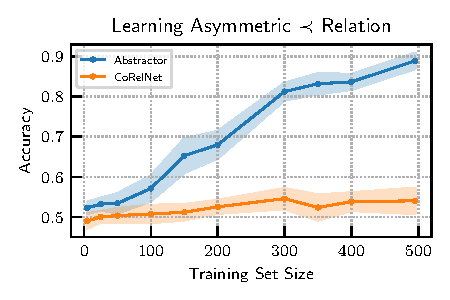
\includegraphics{figures/experiments/pairwise_order_learning_curves.pdf}
        \caption{The Abstractor learns the transitive $\prec$ relation and generalizes, whereas CorelNet's learning curve is flat at the baseline accuracy of 0.5.}\label{fig:exp_order_relation}
    \end{subfigure} \hspace{\fill}
    \begin{subfigure}[t]{0.45\textwidth}
        %\centering
        \hskip-.3in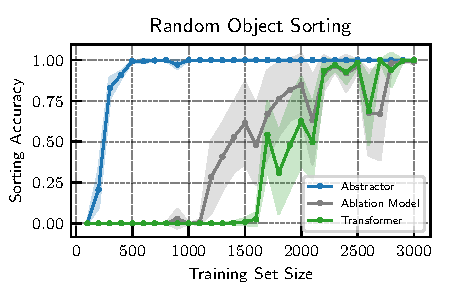
\includegraphics{figures/experiments/random_object_sorting.pdf}
        \caption{Learning curves on sorting sequences of random objects. The abstractor is dramatically more sample-efficient.}\label{fig:exp_object_sorting}
    \end{subfigure}

    \bigskip
    \begin{subfigure}[t]{0.45\textwidth}
        %\centering
        \hskip-.3in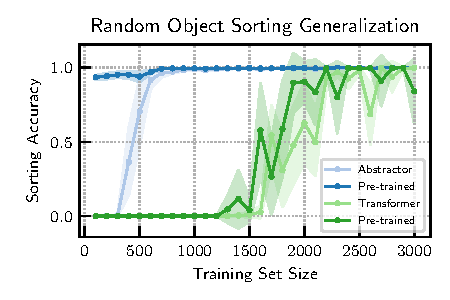
\includegraphics{figures/experiments/random_object_sorting_generalization.pdf}
        \caption{Learning curves with and without pre-training on a similar sorting task. The Abstractor benifits significantly from pre-training whereas the Transformer does not.}\label{fig:exp_object_sorting_generalization}
    \end{subfigure} \hspace{\fill}
    \begin{subfigure}[t]{0.45\textwidth}
        %\centering
        \hskip-.3in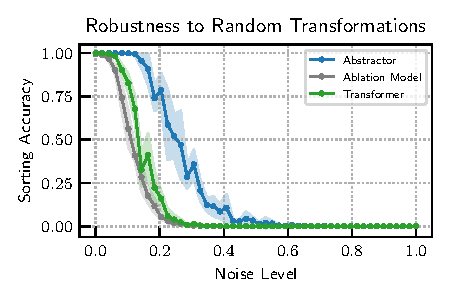
\includegraphics{figures/experiments/multiplicative_robustness.pdf}
        \caption{The Abstractor is more robust to corruption by a random linear transformation.}\label{fig:exp_robustness}
    \end{subfigure}
    \caption{Experiments. Shaded regions indicate twice the standard error of mean, computed over several trials.}\label{fig:experiments}
\end{figure}


\subsection{Warm up: Ability to learn asymetric and multi-dimensional relations}
One recent work on relational machine learning is~\cite{corelnet}, where the authors argue for a particular type of inductive bias in relational models and propose CorelNet. The architecture is very simple: given a sequence of objects $(x_1, ..., x_m)$, embed them using an MLP $\phi$, then compute the similarity matrix $A = \left[\langle\phi(x_i), \phi(x_j)\rangle\right]_{ij}$. The final output is an MLP applied to the flattened similarity matrix. They demonstrate that this model can solve a series of simple tasks with high sample-efficiency compared to models like [transformers and ESBN]. However, CorelNet has several significant limitations. One is that it is only able to model symmetric relations---$A$ is symmetric by definition. Another limitation is that it can only model single-dimensional relations---for each pair of objects $(i,j)$, their modeled relation is a single-dimensional scalar $A_{ij}$. The Abstractor is able to model a significantly larger class of relations. In particular, it is able to model asymetric and multi-dimensional relations through the $\text{MultiHeadRelation}$ operation. This is demonstrated by the following simple experiment (as well as the experiments proceeding it).

We generate $N = 32$ ``random objects'' represented by iid Gaussian vectors, $o_i \overset{iid}{\sim} \mathcal{N}(0, I_d) \in \mathbb{R}^d$, and associate an order relation to them $o_1 \prec o_2 \prec \cdots \prec o_N$. We train several different relational models to learn this order relation. Note that $\prec$ is \textit{not symmetric}. Of the $N^2 = 1024$ possible pairs $(o_i, o_j)$, 35\% are held out as a test set and 15\% are held out as a validation set (for early stopping). We evaluate learning curves by training on the remaining 50\% and computing accuracy on the test set. Note that under this set up, we are evaluating the models on pairs they have never seen. Thus, the models will need to generalize based on the transitivity of the $\prec$ relation.

The Abstractor model follows~\cref{alg:...} with \texttt{num\_layers=1, rel\_dim=4, symbol\_dim=64, proj\_dim=16}. CorelNet uses a dense layer as the embedder $\phi$. The same two-layer MLP is used as the final classification layer in both models. We observe that a simple Abstractor model is able to learn the relation while CorelNet cannot~\cref{fig:exp_order_relation}

\subsection{Superior sample-efficiency on relational tasks compared to plain transformers}
The next experiment extends the idea of learning an order relation $\prec$ on random objects: now, the task is to fully sort sequences of randomly permuted random objects.

We generate random objects in the following way. First, we generate two sets of random attributes $\mathcal{A} = \{a_1, a_2, a_3, a_4\}$, $a_i \overset{iid}{\sim} \mathcal{N}(0, I) \in \mathbb{R}^{4}$ and $\mathcal{B} = \{b_1, \ldots, b_{12}\}$, $b_i \overset{iid}{\sim} \mathcal{N}(0, I) \in \mathbb{R}^{8}$. To each set of attributes, we associate the strict ordering relation $a_1 \prec a_2 \prec a_3 \prec a_4$ and $b_1 \prec b_2 \prec \cdots \prec b_{12}$, respectively. Our random objects are formed by the cartesian product of these two attributes $\mathcal{O} = \mathcal{A} \times \mathcal{B}$, yielding $N = 4 \times 12 = 48$ objects (i.e.: each object in $\mathcal{O}$ is a vector in $\mathbb{R}^{4+8}$ formed by a concatenation of one attribute value in $\mathcal{A}$ and one in $\mathcal{B}$). Then, we associate with $\mathcal{O}$ the strict ordering relation corresponding the order relation $\mathcal{A}$ as the primary key and the order relation of $\mathcal{B}$ as the secondary key. i.e.: $(a_i, b_j) \prec (a_k, b_l)$ if $a_i \prec a_k$ or if $a_i = a_k$ and $b_j \prec b_l$.

Given, a set of objects in $\mathcal{O}$, the task is to sort it according to $\prec$. More precisely, the input sequences are randomly permuted sequences of $10$ objects in $\mathcal{O}$ and the target sequences are the indices of the object sequences in sorted order (i.e., the `argsort'). The training data are sampled uniformly from the set of length-10 sequences in $\mathcal{O}$. We also generate a non-overlapping validation dataset (used during training for early stopping) and a testing dataset (used during evaluation).

We evaluate learning curves on an Abstractor, a Transformer, and an ``Ablation'' model. The Abstractor uses the architecture $\texttt{Encoder} \to \texttt{Abstractor} \to \texttt{Decoder}$. The Encoder-to-Abstractor interface uses relational cross-attention and the Abstractor-to-Decoder interface uses standard cross-attention. The Ablation Model aims to test the effects of the relational cross-attention in the Abstractor model---it is architecturally identical to the Abstractor model with the crucial exception that the Encoder-to-Abstractor interface instead uses standard cross-attention. The hyperparameters of the models are choosen so that the parameter counts are similar. % TODO: add details here? or in supplement?

We find that the Abstractor is dramatically more sample-efficient the Transformer and the Ablation model~\cref{fig:exp_object_sorting}.

\subsection{Modularity and ability to generalize to similar tasks}

Continuing with the object-sorting task and the dataset generated as described above, we test the Abstractor's ability to generalize from similar relational tasks through pre-training. The main task uses the same dataset described above. The pre-training task involves the same object set $\mathcal{O}$ but the order relation is changed. The ordering in attribute $\mathcal{A}$ is randomly permuted, while the ordering in attribute $\mathcal{B}$ is kept the same. A strict ordering relation $\prec$ on $\mathcal{O}$ is obtained in the same way---using the order in $\mathcal{A}$ as the primary key and the order in $\mathcal{B}$ as the secondary key.

The Abstractor model here uses the architecture $\texttt{Abstractor} \to \texttt{Decoder}$ (i.e.: no Transformer encoder), and the transformer is the same as the previous section. We pre-train both models on the pre-training task then evaluate learning curves on the original task with weights initialized to be those learned on the pre-training task. Since the Transformer requires more training samples to learn the object-sorting task, we use a pre-training set size of $3,000$, chosen based on the results of the previous subsection so that it is large enough for the Transformer to learn the pre-training task. This experiment assesses the models' ability to generalize relations learned on one task to a new task which is similar. ~\cref{fig:exp_object_sorting_generalization} shows the learning curves for each model with and without pre-trainign. We observe that when the Abstractor is pre-trained, its learning curve on the object-sorting task is significantly accelerated. The transformer does not benifit from pre-training.

\subsection{Robustness and Out-of-Distribution generalization}
In this experiment, we evaluate robustness to a particular type of noisy corruption. We train each model on the same object-sorting task in the previous two subsections. We use a fixed training set size of $3,000$ for the same reason---it is large enough that all models are able to learn the task. On the hold out test set, we corrupt the object representations by applying a random linear transformation. In particular, we randomly sample a random matrix whose entries are iid zero-mean Gaussian with variance $\sigma^2$, $\Phi \in \mathbb{R}^{d \times d}, \Phi_{ij} \sim \mathcal{N}(0, \sigma^2)$. Each object in $\mathcal{O}$ is then corrupted by this random linear transformation,
\[\tilde{o}_i = \Phi o_i, \ \text{ for each } i \in [48]\]

The models are evaluated on the hold-out test set with objects replaced by their corrupted version. We evaluate the sorting accuracy of each model while varying the noise level $\sigma$. The results are shown in~\cref{fig:exp_robustness}. We emphasize that the models are trained only on the original objects in $\mathcal{O}$, and are not trained on objects corrupted by any kind of noise.

This experiment can be interpreted in two lights: the first is robustness to noise. The second is a form of out-of-distribution generalization. Note that the objects seen by the models post-corruption lie in a different space to those seen during training. However, their relations remain the same. Hence, the models need to learn relations that are in some sense independent of representation.

There is a theoretical justification for this behavior.~\cite{zhouCompressedPrivacySensitive2009} shows that $\langle \Phi x, \Phi y \rangle \approx \langle x, y \rangle$ in high dimensions, for a random matrix $\Phi$ with iid Gaussian entries. Hence, this indicates that models whose primary computations are performed via inner products, like Abstractors, may be more robust to this kind of corruption.

\subsection{Modularity and comparison to purely symbolic representations}
\label{ssec:set_exp}


\begin{wrapfigure}{R}{0.25\textwidth}
	\vskip-5pt
	\begin{tabular}{c}
		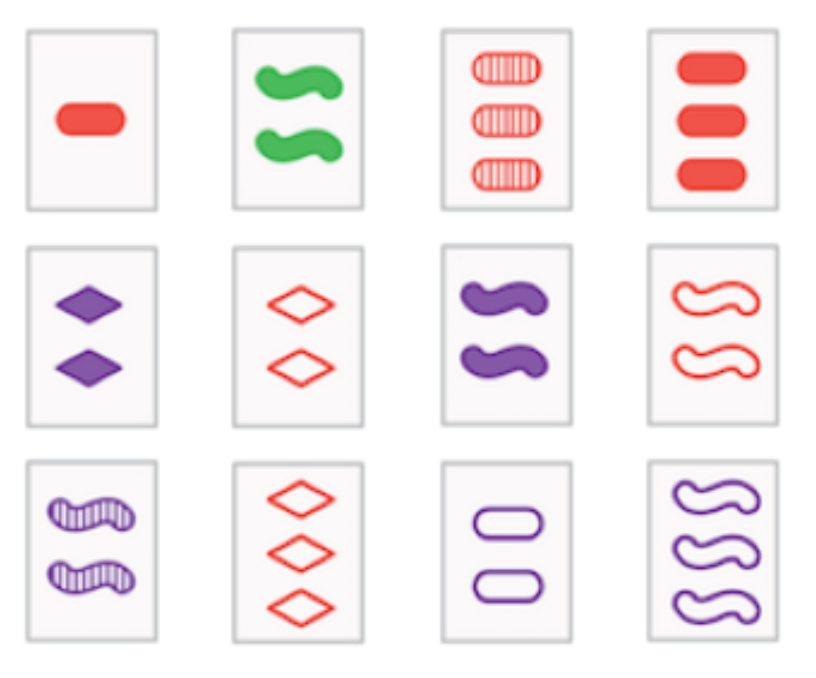
\includegraphics[width=.25\textwidth]{figures/set_example}\\[-5pt]
	\end{tabular}
	\caption{\footnotesize The SET game}
\end{wrapfigure}
SET is a relatively straightforward but challenging cognitive task that engages reasoning faculties in a deliberative
, attentionally directed manner, requiring several levels of abstraction over sensory embeddings. Players are
presented with 12 cards, each of which contains figures that vary along four dimensions (color, number, pattern, and
shape) and they must find subsets of three cards which obey a deceptively simple rule: along each dimension, all cards in a SET must either have the same or unique values.
% JDC: DO FIGURES NEED TO BE NUMBERED?
For example, in the figure to the right, the cards with two solid blue/purple diamonds, two striped blue squiggles, and two open blue oblongs form a SET: same color, same number, different patterns, different shapes.

To simulate the task of deciding if a triple forms a SET, we first train a convolutional neural network to process the color images of the cards (a full deck includes 81 cards). The CNN is trained to predict the attribute of
each card, as a multi-label classification, and then an embedding of dimension $d=32$ of 
each card is obtained. This embedding layer uses an \MLP{} to map the convolutional feature maps into a distributed
representation. Next, we train Abstractors separately for each of the four attributes to learn same/different
relations, where the task is to decide if an input pair of cards is the same or different for that attribute. 
We then use the query and key mappings $W_Q$ and $W_K$ learned for these relations to initialize the relations
in a multi-head Abstractor. The Abstractor is then trained on a dataset of triples of cards, half of which form a SET. 

This is compared to a baseline symbolic model where, instead of images, the input is a vector with 12 bits,
explicitly encoding the relations. That is, for each of the four attributes, a binary symbol is computed for each pair of three input cards---1 if the pair is the same in that attribute, and 0 otherwise. A two-layer MLP is then trained to decide if the triple forms a SET. The MLP using the symbolic representation can be considered as a lower bound on the performance achievable by the Abstractor. This comparison shows that the Abstractor is able to solve a task using relations learned in other tasks (modularity), with a sample efficiency that is not far from that obtained
with purely symbolic, noise-free encodings of the relevant relations. %We note that this uses a simple Abstractor configuration, without self-attention.

% JDC: I REALIZE WE ARE TIGHT ON SPACE, BUT IF THERE IS ROOM, COULD ADD THE FOLLOWING, OR A SHORTENED FORM OF
This subtask suggets how Abstractors might be viewed as an intermediate between strong ``nativist'' approaches that assume a pre-existing foundation of symbolic primitives and purely ``empiricist'' approaches that assume
similar capabilities can emerge simply from processing large amounts of data \cite{howtogrowamind}.
%can be achieved simply by the application of general purpose learning algorithms to large
%amounts of data -- showing how the latter, agumented with simple architectural inductive biases and trained using
%plausible and practical forms of curricular learninng both to generate genuinely symbolic representations, and use these to achieve the flexibilty and efficiency characteristic of human reasoning.
\footnote{We ran the experiments described here on RTX 2080ti, RTX 3090, and A100 GPUs which we had available to us via our institute's internal cluster. The models here are relatively small; powerful GPUs are not required to train a single model. We found the use of GPUs useful for evaluating learning curves over several trials.}